%! TeX program = lualatex
%---------------------------ALLGEMEINE IMPORTS-------------------------------------
\documentclass[12pt,english,ngerman]{scrartcl}
\input{protokoll_template/template.latex/input/shared_preamble.tex}

% Kopfzeile
\ihead{SS24\\
	19.04.2024}

\chead{\textsc{Stark} Matthias --- 12004907 \\
	\textsc{Philipp} Maximilian --- 11839611}

\ohead{Research Lab \\
	Light Tweezers}

% Fußzeile
%\addbibresource{AdvancedMicroscopy.bib}
%todo bib

\usepackage{luacode}

\DeclareSIUnit\px{px}
\DeclareSIUnit\strich{|||}
\DeclareSIUnit\Var{var}
\DeclareSIUnit\VA{VA}
\DeclareSIUnit\bar{bar}

\usepackage{cleveref}

\crefname{enumerate}{Aufzählung}{Aufzählungen}

\begin{document}

\begin{luacode*}
dofile("createExtraPDF.lua")
\end{luacode*}

% \includepdf{./deckblatt.pdf}
\tableofcontents

\newpage

\section{Tasks}\label{Auf}

During the experiment the following steps need to be performed:

\begin{itemize}
	\item Build a microscope and observe forces on microscopic particles without a laser
	\item Use the laser as a "gun"\  to hit some microscopic particles
	\item Trap particles with the laser beam
	\item Trap "living" \ organisms
	\item Transfer a angular momentum to a particle
\end{itemize}

\section{Grundlagen}\label{Grund}

% todo bitte mit ai

\section{Experimental Setup}\label{sec:versuchsanordnung}

The total setup of the experiment is visible in \autoref{fig:aufbau}. Im general it depends on several cage modules, 
that were used for the single steps.

\begin{figure}[H]
	\begin{center}
		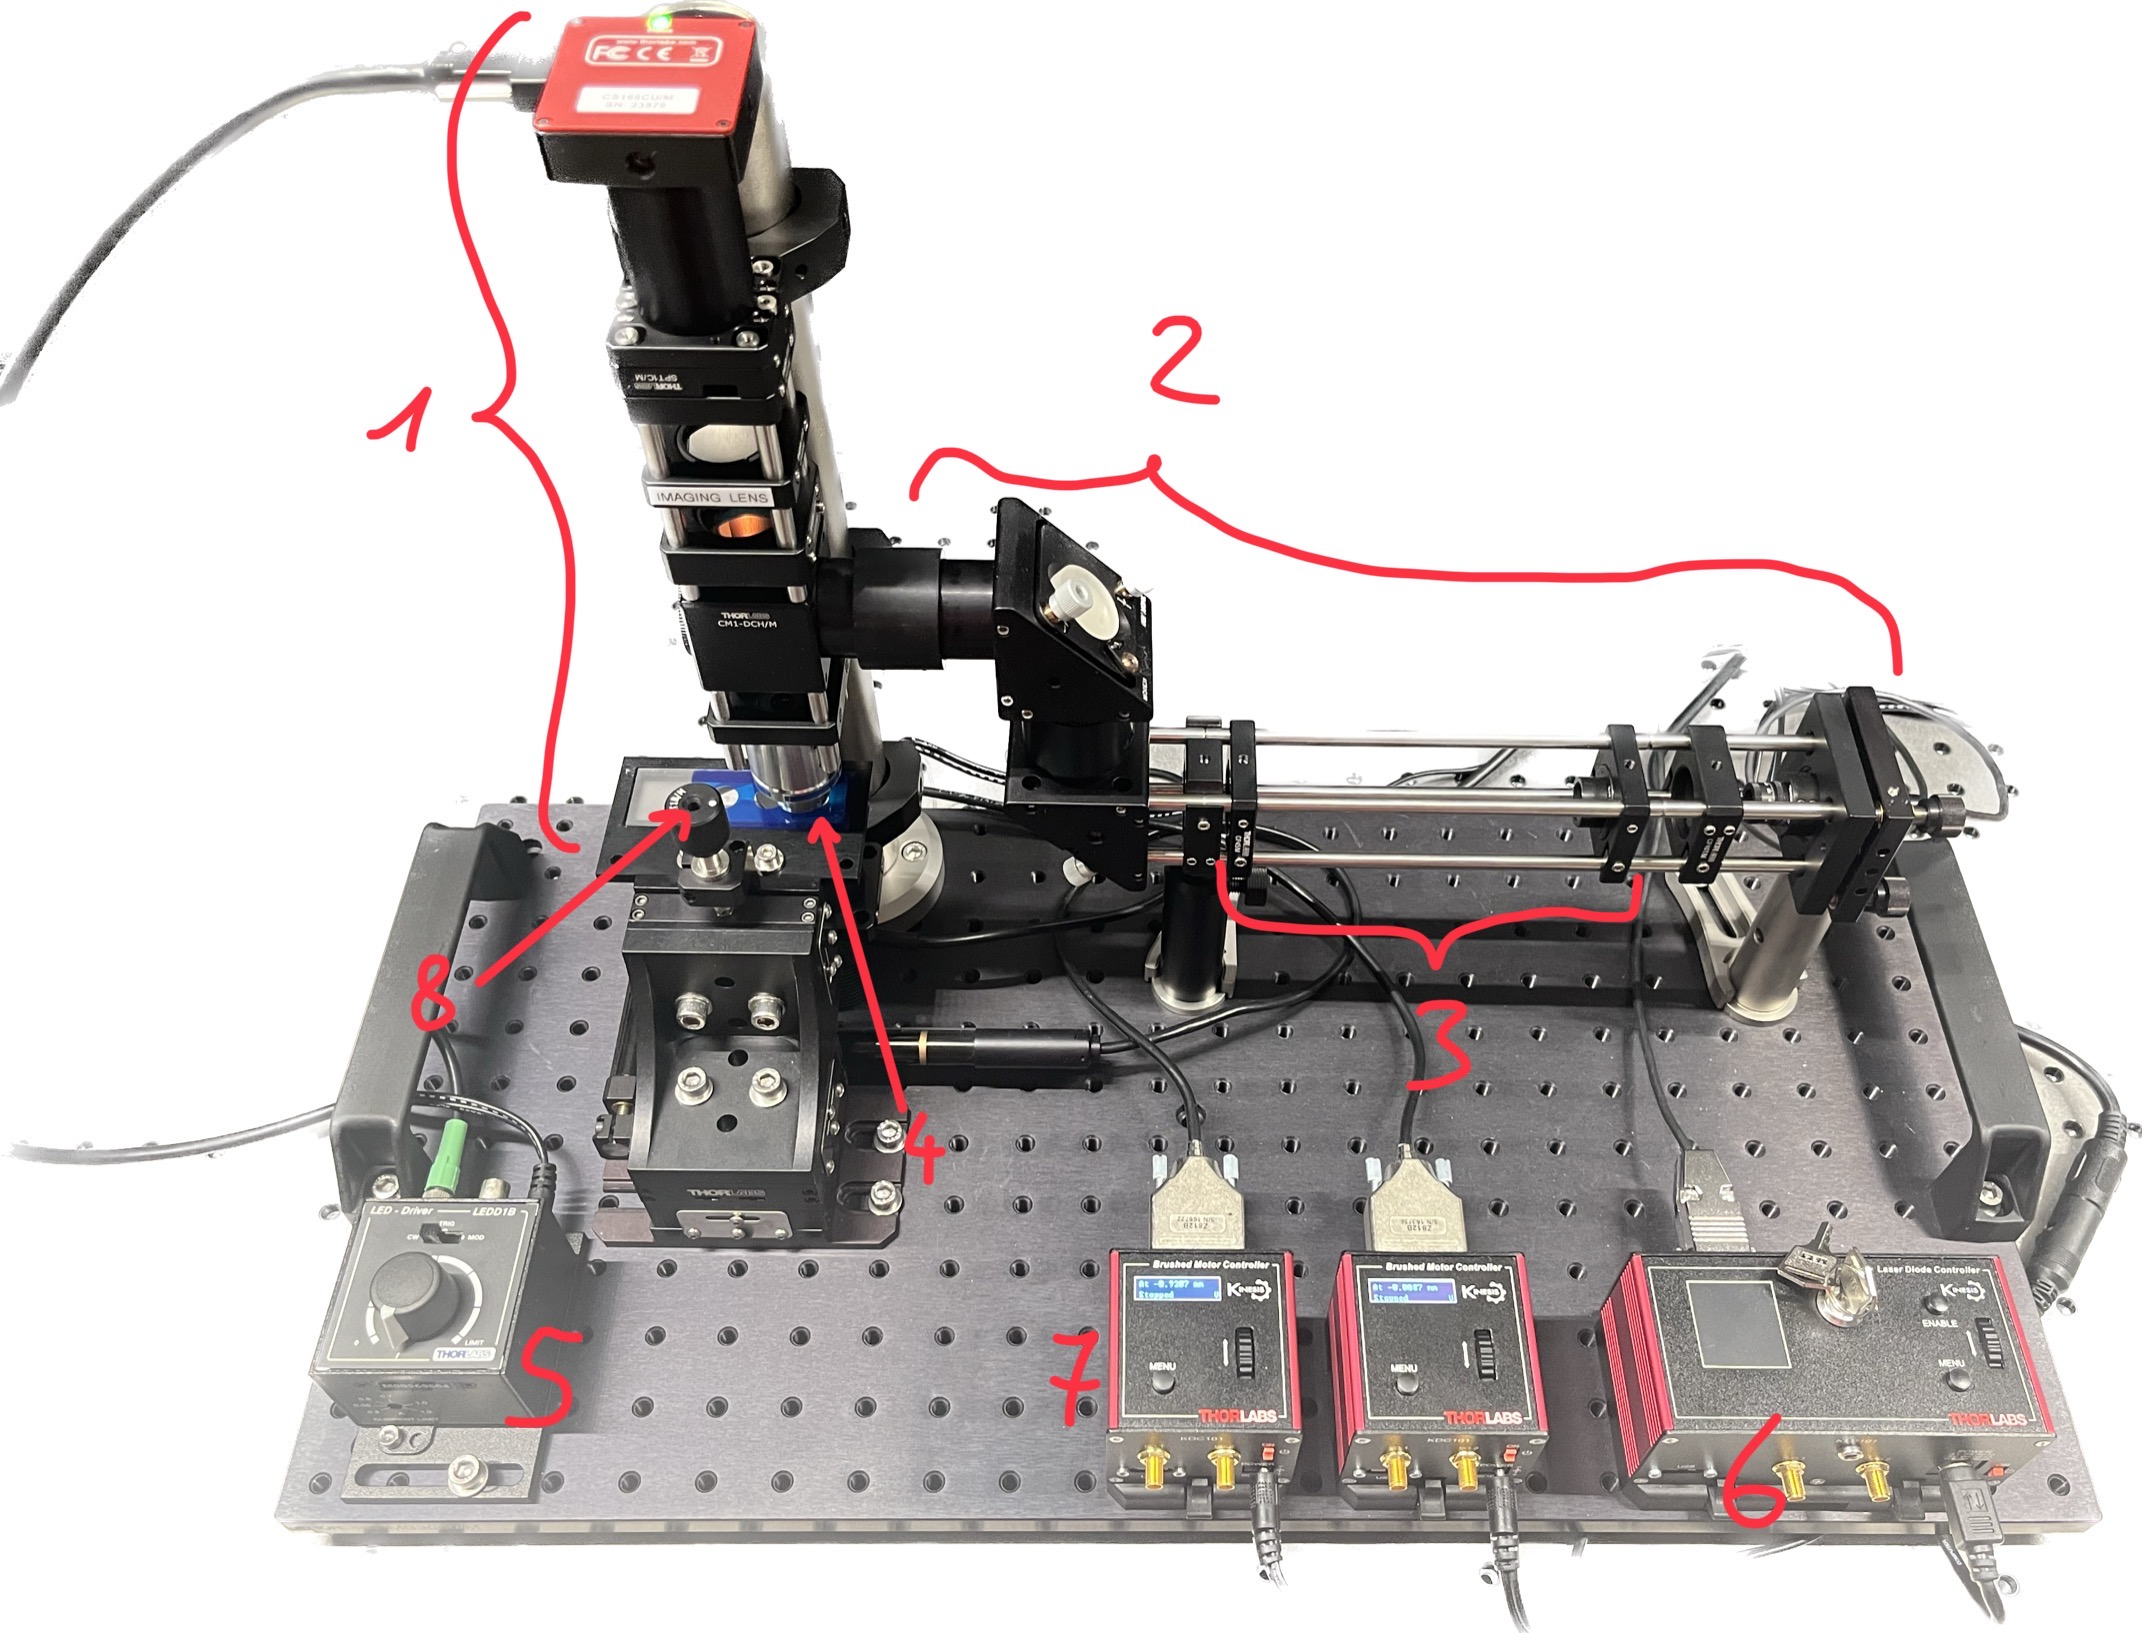
\includegraphics[width =0.7\textwidth]{./figures/aufbau.jpg}
	\end{center}
	\caption[Total experimental setup] {
		Total experimental setup \\
		1 \dots Microscope module               \\
		2 \dots Laser module                                                 \\
		3 \dots Telescope module \\
		4 \dots Sample stage \\
		5 \dots Power supply for light\\
		6 \dots Power supply for laser\\
		7 \dots Controller for movement of the sample in x/y-direction\\
		8 \dots Screw for movement of the sample in z-direction
	}\label{fig:aufbau}
\end{figure}

The single optical components, as well as the beampath are visible in \autoref{fig:aufbau_banzer}.

\begin{figure}[H]
	\begin{center}
		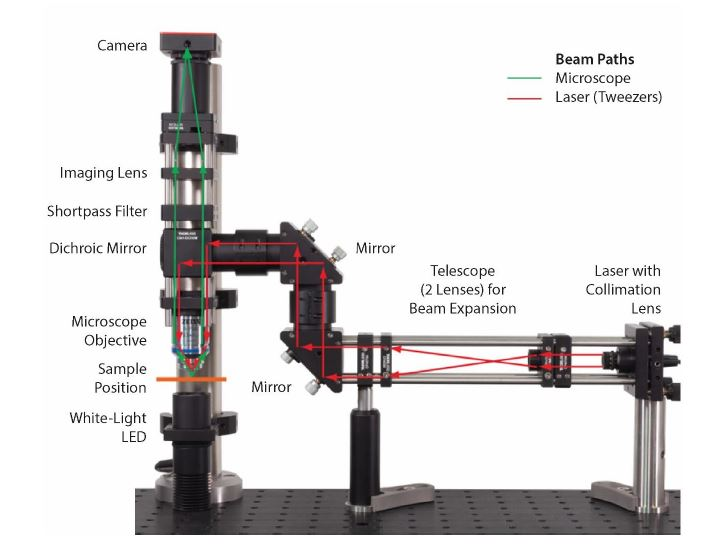
\includegraphics[width =0.9\textwidth]{./figures/aufbau_banzer.JPG}
	\end{center}
	\caption[Optical setup] {
		Optical setup with drawn beampath %todo \cite{unterlagen}
	}\label{fig:aufbau_banzer}
\end{figure}



\section{Materials}\label{sec:geraeteliste}

For the setup the following parts in \autoref{tab:gerate} are used.

%todo

\begin{table}[H]
	\begin{center}
		\caption{Verwendete Geräte für die Abbildung durch eine Sammellinse
		}
		\begin{tblr}{cells={font=\footnotesize},colspec={lllll}}
			\textbf{Gerätetyp}               & \textbf{Hersteller} & \textbf{Typ} & \textbf{Anmerkung} \\
			Linse                            &                     &              & zu bestimmen       \\
			Lens Mount                       & ThorLabs            & LMR1/M       &                    \\
			Optical Posts                    & ThorLabs            & TR3          &                    \\
			Rail Carrier                     & ThorLabs            & XT34TR1/M    & 3x                 \\
			Halogenlampe                     & ThorLabs            & QTH10/M      &                    \\
			Mount for Rectangular Optics     & ThorLabs            & XYF1/M       &                    \\
			Resolution and Distortion Target & ThorLab             & R1L3S5P      &                    \\
			Aluminium-Schiene                &                     &              &                    \\
			Schirm                           &                     &              & selbst gebaut      \\
			Schibelehre                      & Workzone            & 819547       & digital            \\
		\end{tblr}\label{tab:gerate}
	\end{center}
\end{table}



\section{Implementation and Measurement}\label{sec:versuchsdurchfuehrung_messergebnisse}

\subsection{Microscope}

\subsection{Lasergun}


\subsection{Trapping with laser}


\subsection{Trapping of living organisms}


\subsection{Transfer of angular momentum}



\section{Auswertung}\label{sec:auswertung}

Um zu sehen wie sich die Unsicherheit der Messungen bis in die Ergebnisse
fortpflanzt, ist erweiterte Gauss-Methode verwendet worden. Die Grundlagen
dieser Methode stammen von den Powerpointfolien von
% GUM~\cite{wolfgang_kessel_isobipm-gum_2004}. Für die Auswertung ist die
Progammiersprache Python im speziellen die Pakete \verb#labtool-ex2#,
\verb#pandas#, \verb#sympy#, \verb#lmfit# zur Hilfe genommen worden.
\verb#lmfit# wurde für das Fitten verwendet, \verb#sympy# wurde für symbolische
Manipulation verwendet und die restlichen Pakete für leichteres Handhaben der
Daten. Dies wurde aber alles durch \verb#labtool-ex2# abstrahiert.

Um höchstmögliche Genauigkeit zu garantieren wird erst bei der Darstellung der
Wert in Tabellen gerundet.


\subsection{Microscope}

\subsection{Lasergun}


\subsection{Trapping with laser}


\subsection{Trapping of living organisms}


\subsection{Transfer of angular momentum}





\section{Diskussion}\label{sec:diskussion}

\subsection{Microscope}

\subsection{Lasergun}


\subsection{Trapping with laser}


\subsection{Trapping of living organisms}


\subsection{Transfer of angular momentum}






\section{Zusammenfassung}\label{sec:zusammenfassung}

\subsection{Microscope}

\subsection{Lasergun}


\subsection{Trapping with laser}


\subsection{Trapping of living organisms}


\subsection{Transfer of angular momentum}





\newpage
\printbibliography
%todo literatur
\listoffigures
\listoftables
\end{document}
